\documentclass{article}
\usepackage{pgfplots}

\begin{document}

\begin{figure}
  \centering
  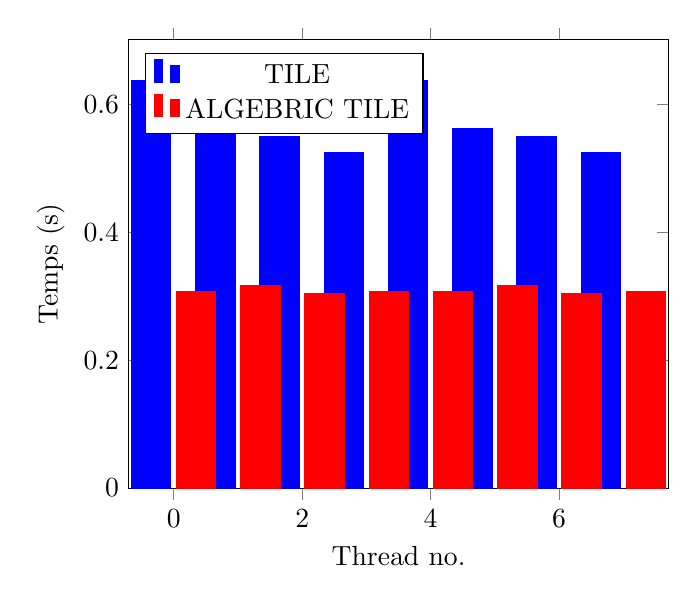
\begin{tikzpicture}
    \begin{axis}[
      ybar,
      bar width=0.5cm,
      xlabel={Thread no.},
      ylabel={Temps (s)},
      ymin=0,
      legend pos=north west
    ]

    % Données pour 2mm.c
    \addplot[color=blue, fill=blue] coordinates {
      (0,0.637530) (1,0.561801) (2,0.549926) (3,0.524434) (4,0.637530) (5,0.561801) (6,0.549926) (7,0.524434)
    };
    \addlegendentry{TILE}

    \addplot[color=red, fill=red] coordinates {
      (0,0.306811) (1,0.316065) (2,0.303637) (3,0.307213) (4,0.306811) (5,0.316065) (6,0.303637) (7,0.307213)
    };
    \addlegendentry{ALGEBRIC TILE}

    \end{axis}
  \end{tikzpicture}
  \caption{Temps d'exécution des threads pour le fichier 2mm.c}
  \label{fig:2mm.c}
\end{figure}

\begin{table}[htbp]
  \centering
  \caption{Statistiques pour le fichier 2mm.c}
  \begin{tabular}{|c|c|c|}
    \hline
    Statistique & Algebraic Tile & Tile \\ 
    \hline
    Skewness (g1) & .86862 & .79745 \\ 
    Kurtosis (g2) & 35.00000 & 30.90719 \\ 
    Écart type & .0421168291 & .0421168291 \\ 
    Percent Imbalance metric en \% & 4.01000 & 19.46600 \\ 
    \hline
  \end{tabular}
\end{table}

\end{document}
